%
% Simpliziale Homologie
%
\section{Simpliziale Homologie
\label{buch:topologie:section:simplex}}
\kopfrechts{Simpliziale Homologie}%
Die von Leonhard Euler entdeckte kombinatorische Eigenschaft der platonischen
\index{Euler, Leonhard}%
Körper lässt sich auf beliebige triangulierte Körper und sogar
\index{platonische Korper@platonischer Körper}%
auf Mannigfaltigkeiten höherer Dimension ausdehnen.
Die Vorgehensweise und die wichtigsten Eigenschaften sollen in den
folgenden Abschnitten skizziert werden.

%
% Zellenkomplexe
%
\subsection{Zellenkomplexe}
Eine Triangulation einer Fläche zerlegt die Fläche in Dreiecke,
Kanten und Punkte.
\index{Triangulation}%
Dabei müssen Ecken und Kanten von benachbarten Dreiecken aufeinander
fallen.
Es ist zum Beispiel nicht zulässig, dass eine Ecke eines Dreiecks
auf einen inneren Punkt einer Kante eines Nachbardreiecks fällt.
Der Begriff des Zellenkomplexes verallgemeinert die Idee
der Triangulation und erlaubt, damit zu rechnen.
\index{Triangulation}%
\index{Zellenkomplex}%

%
% Simplizes
%
\subsubsection{Simplizes}
Punkte, Kanten und Dreieck sind die vertraute Spezialfälle des allgemeinen
\index{Punkt, als $0$-Simplex}%
\index{Kante, als $1$-Simplex}%
\index{Dreieck, als $2$-Simplex}%
Konzeptes eines Simplex.
%
% fig-simplex.tex
%
% (c) 2025 Prof Dr Andreas Müller
%
\begin{figure}
\centering
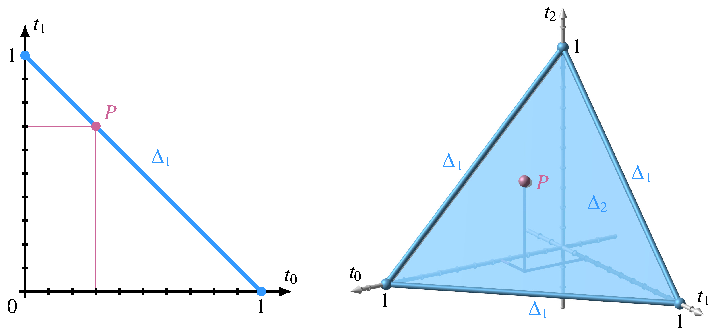
\includegraphics{chapters/120-topologie/images/simplex.pdf}
\caption{Ein- und zweidimensionale Simplizes als Punktmengen in
$\mathbb{R}^{k+1}$ für $k=1,2$.
Die Schnittmengen von $\Delta_2$ mit den Koordinatenebenen bilden
jeweils ein 1-Simplex.
\label{buch:topologie:simplex:fig:simplex}}
\end{figure}
%

\begin{definition}[Simplex]
\index{Simplex}%
Ein \emph{$n$-dimensionales Simplex} ist die Menge
\index{Simplex}%
\index{n-Simplex@$n$-Simplex}%
\[
\Delta_n
=
\{
(t_0,\dots,t_n)
\subset
[0,1]^{n+1}
\mid
t_0+\dots+t_n=1
\}.
\]
\end{definition}

Im Falle $n=0$ besteht $\Delta_0$ nur aus der Zahl $1$.
$\Delta_1$ besteht aus Paaren $(t_0,t_1)$ mit $t_0+t_1=1$, die
als die Strecke zwischen $(1,0)$ und $(0,1)$ visualisiert
werden (Abbildung~\ref{buch:topologie:simplex:fig:simplex} links).
Ebenso besteht die Menge $\Delta_2$ aus den Punkten der Ebene mit
der Gleichung $t_1+t_2+t_3=1$ im postiven Oktanten eines
dreidimensionalen kartesischen Koordinatensystems mit Koordinaten
$t_1$, $t_2$ und $t_3$
(Abbildung~\ref{buch:topologie:simplex:fig:simplex} rechts).

In der Teilmenge
\[
\Delta_{n,i}
=
\{
(t_0,\dots,t_n)
\subset
[0,1]^{n+1}
\mid
t_0+\dots+t_n=1
\wedge
t_i=0
\}
\subset
\Delta_n
\]
sind $n+1$-Tupel, deren $i$-Koordinate verschwindet.
Die Mengen $\Delta_{n,i}$ heissen die \emph{Seitenflächen}
\index{Seitenflache@Seitenfläche}%
des Simplex $\Delta_n$.

Für die verbleibenden Koordinaten gilt wegen $t_i=0$ ebenfalls
\[
t_0+\dots+t_i+\dots+t_n
=
t_0+\dots+\widehat{t_i}+\dots+t_n
=
1,
\]
wobei der Hut bedeutet, dass dieser Term weggelassen wird.
Man kann die Menge also durch die Abbildung
\[
\iota_i
\colon
\Delta_{n-1}
\to
\Delta_{n,i}
:
(t_0,\dots,t_{n-1})
\mapsto
(t_0,\dots,0,\dots,t_{n-1})
\]
parametrisieren.
Die Abbildung $\iota_i$ ist bijektiv, stetig und die Umkehrung ist
ebenfalls stetig.
Die Seitenflächen $\Delta_{n,i}$ sind also Simplizes kleinerer 
Dimension.

Zwei Seitenflächen eines Simplex stossen in einer Menge zusammen,
die ein Simplex der Dimension $n-2$ ist.
Die gemeinsamen Punkte der beiden Seitenflächen $\Delta_{n,i}$ und
$\Delta_{n,k}$ bilden die Menge
\[
\Delta_{n,ik}
=
\{
(t_0,\dots,t_n)
\mid
t_0+\dots+t_n=1
\wedge
t_i=0
\wedge
t_k=0
\},
\]
die sich nach dem gleichen Muster wie die Seitenfläche mit der Menge
$\Delta_{n-2}$ identifizieren lässt.

\begin{definition}[Zellenkomplex]
\index{Zellenkomplex}%
Ein \emph{Zellenkomplex} ist ein topologischer Raum, der durch
Zusammenfügen von endlich vielen Simplizes entlang von Untersimplizes
kleinerer Dimension entsteht.
\index{Dimension}%
Die \emph{Dimension} eines Zellenkomplexes ist die höchste Dimension
der Simplizes, aus denen er besteht.
\end{definition}

Ein Zellenkomplex der Dimension $n$ setzt sich also aus maximal
$n$-dimensionalen Simplizes zusammen, die Seitenflächen oder
Simplizes noch kleinerer Dimension gemeinsam haben können.

%
% Euler-Charakteristik eines Zellenkomplexes
%
\subsubsection{Euler-Charakteristik eines Zellenkomplexes}
Eulers Entdeckung bezog sich auf Polyeder, die sich natürlich nur
aus Ecken, Kanten und Flächen, also Simplizes der Dimension 0, 1
bzw.~2.
Bezeichnen wir die Anzahl der $k$-dimensionalen Simplizes mit $t_k$,
dann wird die von Euler berachtete Summe 
\begin{align*}
E - K + K
&=
t_0
-
t_1
+
t_2,
\intertext{die wir auch}
&=
\sum_{k=0}^2 (-1)^kt_k
\end{align*}
schreiben können.
Diese Schreibweise lässt sich leicht auf beliebige Dimension
verallgemeinern.

\begin{definition}[Euler-Charakteristik]
Sei $S$ ein $n$-dimensionaler Zellenkomplex in dem
genau $k_i$ Simplizes der Dimension $i$ vorkommen.
Dann ist die Summe
\[
\chi(S)
=
k_0 - k_1 + \dots + (-1)^n t_n
=
\sum_{i=0}^n (-1)^i k_i
\]
die \emph{Euler-Charakteristik} von $S$.
\index{Euler-Charakteristik}%
\index{Euler-Charakteristik!eines Zellenkomplexes}%
\end{definition}

%
% Verfeinerung eines Zellenkomplexes
%
\subsubsection{Verfeinerung eines Zellenkomplexes}
Die Definition der Euler-Charakteristik hängt von der Triangulation ab.
Wir müssen daher zeigen, dass eine Verfeinerung eines Zellenkomplexes die
Euler-Charakteristik nicht ändert.
Statt eines vollständigen Beweises dieser Eigenschaft zeigen wir anhand
einiger illustrativer Beispiele, was sich bei der Verfeinerung
abspielt.
%
% fig-unterteilung.tex
%
% (c) 2025 Prof Dr Andreas Müller
%
\begin{figure}
\centering
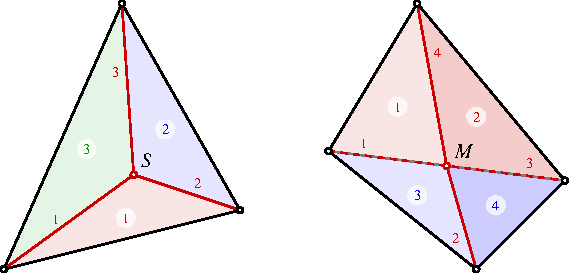
\includegraphics{chapters/120-topologie/images/unterteilung.pdf}
\caption{Links: Bei der Unterteilung eines einzelnen Dreiecks durch einen
inneren Punkt $S$ entstehen drei Dreieck ($2$ mehr also vor der Unterteilung)
und 3 neue Kanten.
Rechts: Bei der Unterteilung der Kante $AB$ durch den Punkt $M$ werden
\index{Unterteilung}%
beide Nachbardreiecke (rot und blau) in jeweils zwei Dreiecke
($2$ mehr als vor der Unterteilung)$ zerlegt.
Ausserdem entstehen drei zusätzliche Kanten.
In allen Fällen ändert sich die Euler-Charakteristik nicht.
\label{buch:topologie:eulercharakteristik:fig:unterteilung}}
\end{figure}
%

Wir beginnen mit einem zweidimensionalen Zellenkomplex
und betrachten ein einzelnes Dreieck.
Der Zellenkomplex kann verfeinert werden, indem im Inneren des
Dreiecks ein weiterer Punkt hinzugefügt wird
(Abbildung~\ref{buch:topologie:eulercharakteristik:fig:unterteilung} links).
Neue Kanten vom neuen Punkt zu den Ecken des Dreiecks ergeben die
verfeinerte Triangulation.
Die Triangulation bekommt also eine zusätzliche Ecke, drei zusätzliche
Kanten und aus einem Dreieck werden drei, also zwei zusätzliche Dreiecke.
Für die Euler-Charakteristik bekommen wir daher
\[
(E+1) - (K+3) - (F+2)
=
E-K+F+(\underbrace{1-3+2}_{\displaystyle=0})
=
E-K+F,
\]
die Euler-Charakteristik ändert also nicht.

Unterteilt man eine Kante mit einem neuen Punkt, dann müssen auch
die angrenzenden beiden Dreiecke mit einer Kante zur gegenüberliegenden
Ecke neu unterteilt werden
(Abbildung~\ref{buch:topologie:eulercharakteristik:fig:unterteilung} rechts).
Die Anzahl der Ecken vergrössert sich um eins.
Aus der ursprünglichen Kante werden zwei und es kommen zwei neue Kanten
dazu.
Die Anzahl der Dreiecke wächst um zwei.
Die Euler-Charakteristik ist neu
\begin{align*}
(E+1) - (K+3) - (F+2)
=
E-K+F +(\underbrace{1-3+2}_{\displaystyle=0})
=
E-K+F,
\end{align*}
sie verändert sich also auch bei Unterteilung einer Kante nicht.

In drei Dimensionen wird die Unterteilung etwas komplizierter.
Ein zusätzlicher innerer Punkt in einem Tetraeder zerlegt
es in vier Tetraeder mit dem neuen Punkt als Spitze und den
Seitenflächen des ursprünglichen Tetraeders als Grundfläche.
Für jede ursprüngliche Kante entsteht eine neue Fläche und
für jede ursprüngliche Ecke eine neue Kante.
Die Euler-Charakteristik wird daher zu
\begin{align*}
(E+1) - (K+4) + (F+6) - (V+3)
&=
E-K+F-V
+
(\underbrace{1-4+6-3}_{\displaystyle=0})
\\
&=
E-K+F-V
=
\chi(M),
\end{align*}
bleibt daher unverändert.

Unterteilt man eine Dreiecksfläche durch einen inneren Punkt,
müssen auch die beiden benachbarten Tetraeder unterteilt werden.
Dabei entstehen fünf neue Kanten, sechs neue Flächen und vier
neue Tetraeder.
Die neue Euler-Charakteristik ist daher
\begin{align*}
(E+1) - (K+5) + (F+8) - (V+4)
&=
E-K+F-V
+(\underbrace{1-5+8-4}_{\displaystyle=0})
\\
&=
E-K+F-V
=
\chi(M),
\end{align*}
ebenfalls unverändert.

Schliesslich betrachten wir den Fall der Unterteilung einer Kante,
die $n$ Tetraedern gemeinsam ist, mit $f$ Seitenflächen, die sich
in der Kante treffen.
Durch die Unterteilung wird aus jeder Seitenfläche zu zweien
mit einer zusätzlichen Kante.
Zusätzlich entsteht in jedem ursprünglichen Tetraeder ein zusätzliches
Dreieck mit der gegenüberliegenden Kante als Basis und der neuen
Ecke als Spitze.
Die Zahl der Tetraeder erhöht sich ebenfalls um $n$.
Die neue Euler-Charakteristik ist
\begin{align*}
(E+1)
-
(K+1+f)
+
(F+f+n)
-
(V+n)
&=
E-K+F-V + (\underbrace{1-1-f+f+n-n}_{\displaystyle=0})
\\
&=
E-K+F-V
=
\chi(M),
\end{align*}
wieder unverändert.

Dieselbe Art von Rechnung lässt sich auch für Simplizes beliebig hoher
Dimension durchführen.
Ohne auf den detaillierten Beweis einzugehen, können wir schliessen,
dass die Euler-Charakteristik eine Grösse ist, die nicht von der Unterteilung
des Körpers in Simplizes abhängt.
Die Euler-Charakteristik ist also eine topologische Invariante.

%
% Rand
%
\subsubsection{Rand}
%
% fig-rand.tex
%
% (c) 2025 Prof Dr Andreas Müller
%
\begin{figure}
\centering
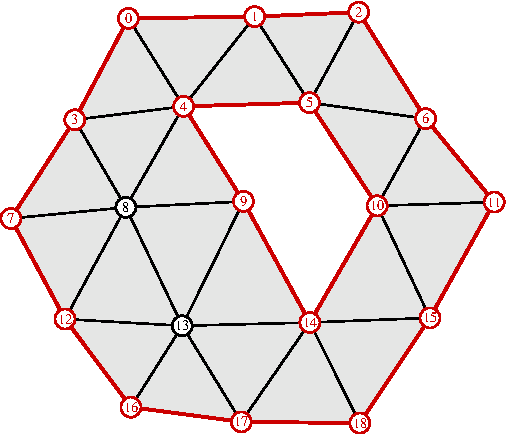
\includegraphics{chapters/120-topologie/images/rand.pdf}
\caption{Rand eines zweidimensionalen simplizialen Komplexes.
\index{Rand}
Die schwarzen Kanten sind innere Kanten und gehören nicht zum Rand.
Nur Kanten, die zu nur einem 2-Simplex gehören, tragen zum Rand bei.
\label{buch:topologie:homologie:fig:rand}}
\end{figure}
%
Ein $n$-Simplex mit den Ecken $p_0\dots p_n$ besteht aus den $(n-1)$-Simplizes,
denen genau eine Ecke fehlt.
Wenn aber zwei $n$-Simplizes entlang eines gemeinsamen $(n-1)$-Simplex
zusammenstossen, dann möchte man dieses nicht als Teil des Randes
des Zellenkomplexes betrachten.
Abbildung~\ref{buch:topologie:homologie:fig:rand} illustriert das Problem.
Die rote eingezeichneten Kanten bilden zusammen den Rand.
Die schwarzen Kanten sind innere Kanten, die jeweils zwei Dreiecken 
gemeinsam sind und nicht zum Rand gezählt werden dürfen.


%
% Homologie
%
\subsection{Kettenkomplexe
\label{buch:topologie:subsection:kettenkomplexe}}
In der linearen Algebra lernt man, dass man ein elektrisches
Netzwerk mit Hilfe von Matrizen beschreiben kann
\cite[Abschnitt~2.A]{buch:linalg}.
Die zum Beispiel für die kirchhoffschen Regeln benötigten Zyklen
im Netzwerk werden beschrieben als Vektoren, deren Komponenten angeben,
welche Kanten zum Zyklus gehören.
Zur Verifikation, dass es sich um einen Zyklus handelt, erfolgt dann
durch Anwendung einer Matrix $\partial$, welche den Endpunkten der
Kanten Zahlen $\pm 1$ zuweist.
Ein Zyklus liegt vor, wenn in der Summe keine Ecke übrig bleibt.
Die Diskussion des Randes am Ende des vorangegangenen Abschnittes
zeigt, dass die Idee des Rechnens mit Ecken mit rellen Koeffizienten 
auf Simplizes beliebiger Dimension ausgeweitet werden muss.
Dabei entsteht das algebraische Konzept eines Kettenkomplexes.

%
% Vektorraum der Simplizes
%
\subsubsection{Vektorraum der Simplizes}
Der Rand eines Simplexes ist nicht ein einzelnes Simplex, sondern
eine Menge von Simplizes.
Genau genommen müssen wir ausserdem auch noch die Orientierung eines
Simplexes berücksichtigen.
Ein zweidimensionales Simplex mit den Ecken $ABC$ hat als Rand
die drei Simplizes $AB$, $BC$ und $AC$, aber das letzte wird in
entgegengesetzter Richtung durchlaufen.

\begin{definition}
Sei $S$ ein $n$-dimensionaler Zellenkomplex.
Für jedes $k$, $0\le k\le n$ ist $C_k$ der reelle Vektorraum aufgespannt
von den Simplizes von $S$.
Die Elemente $c\in C_k$ sind Linearkombinationen von $k$-dimensionalen
Simplizes.
Sie werden auch $k$-dimensionale \emph{Ketten} genannt.
\index{Kette}%
\end{definition}

\begin{beispiel}
\label{buch:topologie:eulercharakteristik:bsp:dreieck}
Wir betrachten den Zellenkomplex, der aus nur einem Dreieck
$\triangle ABC$ besteht.
Die $0$-dimensionalen Simplizes sind die Ecken $A$, $B$ und $C$, 
die eindimensionalen Simplizes sind die Kanten $AB$, $BC$ und $AC$.
Daher sind die Vektorräume $C_k$ gegeben durch
\begin{align*}
C_0 &= \{ x_A A + x_B B + x_C C\mid x_A, x_B, x_C\in\mathbb{R}\}
&
\dim C_0 &= 3
\\
C_1 &= \{ x_{AB} AB + x_{BC} BC + x_{AC} AC\mid x_{AB}, x_{BC}, x_{AC} \in\mathbb{R}\}
&
\dim C_1 &= 3
\\
C_2 &= \{ x_{ABC} ABC\mid x_{ABC}\in\mathbb{R}\}
&
\dim C_2 &= 1.
\qedhere
\end{align*}
\end{beispiel}

%
% Randoperator
%
\subsubsection{Randoperator}
Da wir jetzt beliebige Simplizes linear kombinieren können, können
wir auch den Rand eines Simplex als Linearkombination von
niedrigerdimensionaler Simplizes ausdrücken.

\begin{definition}[Randoperator]
Der $k$-dimensionale Randoperator ist die lineare Abbildung
\[
\partial_k
\colon
C_k \to C_{k-1}
:
P_0\dots P_k
\mapsto
\sum_{i=0}^k
(-1)^i
P_0\dots\widehat{P_i}\dots P_k.
\]
\index{Randoperator}%
\end{definition}

\begin{beispiel}
\label{buch:topologie:eulercharakteristik:bsp:dreieckrand}
Das Beispiel~\ref{buch:topologie:eulercharakteristik:bsp:dreieck}
konstruiert die Vektorräume $C_k$ für ein Dreieck.
\index{Tetraeder}%
Der $0$-dimensionale Randoperator $\partial_0$ ist der Null-Operator.
In höheren Dimension sind Randoperatoren gegeben durch
\begin{align*}
\partial_1 AB &= -B + A &&&&\\
\partial_1 BC &= -C + B &
&\Rightarrow
&\partial_1&=\smash{\begin{pmatrix*}[r]
 1 &  0 &  1 \\
-1 &  1 &  0 \\
 0 & -1 & -1
\end{pmatrix*}}
\\
\partial_1 AC &= -C + A \\
\partial_2 ABC &= AB - AC + BC&&\Rightarrow&\partial_2&=\begin{pmatrix*}[r]1\\1\\-1\end{pmatrix*}
\end{align*}
Als Basis für die Matrixdarstellung der Randoperatoren wird die
Reihenfolge der $k$-Simplizes im
Beispiel~\ref{buch:topologie:eulercharakteristik:bsp:dreieck}
verwendet.

Die gefundenen Randoperatoren wirken zwischen den Vektorräumen $C_k$
wie im Diagramm.
\[
 0                  \xleftarrow{\qquad\clap{$\partial_0=0$}\qquad}
C_0 = \mathbb{R}    \xleftarrow{\qquad\clap{$\partial_1$}\qquad}
C_1 = \mathbb{R}^3  \xleftarrow{\qquad\clap{$\partial_2$}\qquad}
C_2 = \mathbb{R}    \xleftarrow{\qquad\clap{$\partial_3=0$}\qquad}
 0.
\]
Der Rand des Dreiecks ist eine geschlossene Kurve, man erwartet
also, dass der Rand des Randes $0$ ist.
Tatsächlich ist das Produkt der Matrizen 
\begin{align*}
\partial_1\circ\partial_2
=
\begin{pmatrix*}[r]
 1 &  0 &  1 \\
-1 &  1 &  0 \\
 0 & -1 & -1
\end{pmatrix*}
\begin{pmatrix*}[r] 1 \\ 1 \\ -1 \end{pmatrix*}
&=
\begin{pmatrix}0\\0\\0\end{pmatrix}.
\end{align*}
wie erwartet.
\end{beispiel}

\begin{satz}
Der Rand eines Randes verschwindet, $\partial_{k-1}\circ\partial_k=0$.
\end{satz}

\begin{proof}
Da der Randoperator linear ist, muss die Behauptung nur auf $k$-dimensionalen
Simplizes verifiziert werden.
Sei also $\sigma=P_0\dots P_k$ ein $k$-dimensionales Simplex.
Der Randoperator ergibt
\[
\partial_k\sigma
=
\sum_{i=0}^k
(-1)^i P_0\dots\widehat{P_i}\dots P_k.
\]
Die Summanden sind $k-1$-dimensionale Simplizes, deren Rand wir jetzt
zusätzlich ausrechnen müssen.
Dabei müssen erneut Punkte $P_j$ weggelassen und mit einem Vorzeichen versehen
werden.
Da das Vorzeichen von der Position und nicht vom Index abhängt, unterscheiden
wird die Fälle $j<i$ und $j>i$:
\begin{align*}
\partial_{k-1}\partial_k \sigma
&=
\sum_{i=0}^k (-1)^i \partial_{k-1} P_0\dots \widehat{P_i}\dots P_k
\\
&=
\sum_{i=0}^k
\biggl(
\sum_{j=0}^{i-1}
(-1)^{i+j}P_0\dots\widehat{P_j}\dots \widehat{P_i}\dots P_k
+
\sum_{j=i+1}^{k}
(-1)^{i+j+1}P_0\dots\widehat{P_i}\dots \widehat{P_j}\dots P_k
\biggr)
\\
&=
\sum_{j<i}
(-1)^{i+j}P_0\dots\widehat{P_j}\dots \widehat{P_i}\dots P_k
+
\sum_{i<j}
(-1)^{i+j+1}P_0\dots\widehat{P_i}\dots \widehat{P_j}\dots P_k.
\intertext{Vertauschen wir die Namen der Summationsvariablen in der
zweiten Summe und verwandeln wird den Summanden $+1$ im Exponenten
in ein Vorzeichen vor der Summe, entsteht}
&=
\sum_{j<i}
(-1)^{i+j}P_0\dots\widehat{P_j}\dots \widehat{P_i}\dots P_k
-
\sum_{j<i}
(-1)^{i+j}P_0\dots\widehat{P_j}\dots \widehat{P_i}\dots P_k.
\end{align*}
Die beiden Summen heben sich weg, was die Behauptung beweist.
\end{proof}

%
% Kettenkomplex
%
\subsubsection{Kettenkomplex}
Der Randoperator $\partial_k$ ist eine lineare Operation, die den Grad 
erniedrigt.
Ausserdem gilt, dass der iterierte Randoperator verschwindet.
Diese algebraische Struktur tritt auch in anderen Zusammenhängen
auf und verdient daher einen eigenen Namen, der in der folgenden
Definition eingeführt wird.

\begin{definition}[Kettenkomplex]
Eine Folge von Vektorräumen $C_k$ und linearen Abbildungen
$\partial_k\colon C_k\to C_{k+1}$
mit der Eigenschaft $\partial_{k-1}\circ\partial_k=0$ heisst
ein \emph{Kettenkomplex}.
\index{Kettenkomplex}%
Kettenkomplexe werden manchmal auch $(C_*,\partial_*)$ notiert.
\end{definition}

Ein Kettenkomplex $(C_*,\partial_*)$ kann daher auch als Diagramm
\begin{equation}
\dots
\xleftarrow{\;\quad\clap{$\partial_{k-2}$}\quad\;}
C_{k-2}
\xleftarrow{\;\quad\clap{$\partial_{k-1}$}\quad\;}
C_{k-1}
\xleftarrow{\;\quad\clap{$\partial_{k}$}\quad\;}
C_k
\xleftarrow{\;\quad\clap{$\partial_{k+1}$}\quad\;}
C_{k+1}
\xleftarrow{\;\quad\clap{$\partial_{k+2}$}\quad\;}
\dots
\label{buch:topologie:simplex:eqn:kettenkomplex}
\end{equation}
von linearen Abbildung geschrieben werden.
Die Forderung, dass die Verkettung $\partial_{k-1}\circ\partial_k=0$
ist, ist gleichbedeutend mit der Forderung, dass das Bild von $\partial_k$
im Kern von $\partial_{k+1}$ enthalten ist, oder
$\operatorname{im}\partial_k \subset \ker\partial_{k-1}$.
Der Kern von $\partial_{k-1}$ kann aber durchaus grösser sein, es kann
also Elemente $c_{k-1}\in C_{k-1}$ geben mit $\partial_{k-1} c_{k-1}=0$,
für die es kein $c_k\in C_k$ gibt $c_{k-1}=\partial_kc_k$.

\begin{definition}[exakte Folge]
Eine Folge der Form
\eqref{buch:topologie:simplex:eqn:kettenkomplex}
heisst \emph{exakt} an der Stelle $k$, wenn
$\ker\partial_{k} = \operatorname{im}\partial_{k+1}$
gilt.
\end{definition}

\begin{beispiel}
\label{buch:topologie:eulercharakteristik:bsp:dreieckkomplexe}
Für das Dreieck $\triangle ABC$ wurden die Randoperatoren in
Beispiel~\ref{buch:topologie:eulercharakteristik:bsp:dreieckrand}
bereits berechnet.
$\partial_1$ ist eine $3\times 3$-Matrix mit Rang~2, somit ist
\begin{align*}
\dim C_0 &= 3 &
\operatorname{rank} \partial_0 &= 0&
&\Rightarrow&
\dim \operatorname{im}\partial_0 &= 0 &
\dim \ker\partial_0 &= 3
\\
\dim C_1 &= 3 &
\operatorname{rank} \partial_1 &= 2&
&\Rightarrow&
\dim \operatorname{im}\partial_1 &= 2 &
\dim \ker\partial_1 &= {\color{darkred}1}
\\
\dim C_2 &= 1 &
\operatorname{rank} \partial_2 &= 1&
&\Rightarrow&
\dim \operatorname{im}\partial_2 &= {\color{darkred}1} &
\dim \ker\partial_2 &= 0.
\end{align*}
Die beiden roten Zahlen zeigen, dass die Folge an der Stelle $k=1$
exakt ist.

Entfernt man das 2-Simplex $ABC$ aus dem Zellenkomplex, entsteht
ein nur noch eindimensionaler Zellenkomplex.
\begin{align*}
\dim C_0 &= 3 &
\operatorname{rank} \partial_0 &= 0&
&\Rightarrow&
\dim \operatorname{im}\partial_0 &= 0 &
\dim \ker\partial_0 &= 3
\\
\dim C_1 &= 3 &
\operatorname{rank} \partial_0 &= 2&
&\Rightarrow&
\dim \operatorname{im}\partial_1 &= 2 &
\dim \ker\partial_1 &= {\color{darkred}1}
\\
\dim C_2 &= 0 &
\operatorname{rank} \partial_0 &= 0&
&\Rightarrow&
\dim \operatorname{im}\partial_2 &= {\color{darkred}0} &
\dim \ker\partial_2 &= 0.
\end{align*}
Dieser Zellenkomplex ist also nicht mehr exakt an der Stelle $k=1$.
\end{beispiel}

Von besonderem Interesse sind als Kettenkomplexe, die \emph{nicht}
exakt sind.
Die Kettenkomplexe, die aus einem Zellenkomplex abgeleitet
werden, sind oft von dieser Art.
Das Beispiel~\ref{buch:topologie:eulercharakteristik:bsp:dreieckkomplexe}
zeigt, dass ``Löcher'' in einem Zellenkomplex die Exaktheit an einer 
Stelle zerstören können.
Der Begriff der Homologie dient dazu, die Nichtexaktheit zu messen und
damit mit algebraischen Mitteln topologische Information des Zellenkomplexes
zu extrahieren.

%
% Homologie
%
\subsection{Homologie
\label{buch:topologie:simplex:subsection:homologie}}
Der Kettenkomplex zu einem Zellenkomplex ermöglicht, mit Simplizes zu rechnen.
Die Bestimmung des Randes ist eine rein algebraische Operation
in einem Vektorraum geworden.
Damit wird es aber auch einfacher, mit speziellen Teilkomplexen
zu arbeiten, zum Beispiel solchen, die keinen Rand haben, oder solchen,
die als Rand eines Teilkomplexes entstanden sind.

%
% Zyklen und Ränder
%
\subsubsection{Zyklen und Ränder}
Der Randoperator ist ein linearer Operator und wird daher wesentlich
durch Kennzahlen wie Rang und Dimension des Kernes charakterisiert.
Wir geben Kern und Bild des Randoperators spezielle Namen.

\begin{definition}[Zyklen und Ränder]
Die Menge der $k$-dimensionalen {\em Zyklen} ist der Kern
\index{Zyklus}%
\[
Z_k
=
\ker \partial_k 
=
\{ z\in C_k \mid \partial_kz = 0 \}
\]
des Randoperators.
Die Menge der $k$-dimensionalen {\em Ränder } ist das Bild
\index{Rand}%
\[
B_k
=
\operatorname{im} \partial_{k+1}
=
\{ \partial_{k+1}c\mid c\in C_{k+1} \}
\]
des $(k+1)$-dimensionalen Randoperators.
\end{definition}

Da $\partial_{k}\partial_{k+1}=0$ ist, werden Ränder in $B_k$
von $\partial_k$ annihiliert.
Dies bedeutet, dass Ränder immer auch Zyklen sind, dass also
$B_k\subset Z_k$ für alle $k$ gilt.

%
% Homologierelation
%
\subsubsection{Homologierelation}
Die Intuition sagt, dass zwei beliebige Meridiankreise auf dem Torus in
Abbildung~\ref{buch:topologie:intro:fig:torus}
gleichwertig sind.
Das gleiche gilt auch für Merdiane auf der Kugel von
Abbildung~\ref{buch:topologie:intro:fig:sphere}.
Doch wie lässt sich dies mathematisch exakt fassen?
Die Vektorräume der Simplizes bieten eine Möglichkeit.

Zwischen zwei benachbarten Meridiankreisen des Torus befindet sich ein
Streifen von Dreiecken.
Die beiden Merdiankreise sind als der gemeinsame Rand eines 
Teilzellenkomplexes des Torus.
Das gleiche gilt auch für zwei Meridiane auf der Kugel: sie sind
der gemeinsame Rand 

\begin{definition}[homolog]
Zwei Vektoren $a,b\in C_k$ heissen \emph{homolog}, 
\index{homolog}
wenn es ein $c\in C_{k+1}$ gibt mit $\partial c=b-a$.
\end{definition}

Zwei Vektoren heissen also homolog, wenn ihre Differenz ein Rand ist,
wenn also $b-a\in B_k$.
Die Homologierelation ist symmetrisch, denn wenn $\partial c=b-a$ ist,
dann gilt wegen der Linearität $\partial (-c) = -(\partial c)=-(b-a)=a-b$.
Sie ist auch transitiv, denn wenn $a$ und $b$ homolog sind dank
$b-a=\partial d_1$ und $b$ und $c$ dank $c-b=\partial d_2$, dann gilt
für $d=d_1+d_2$
\[
\partial d
=
\partial(d_1+d_2)
=
\partial d_1
+
\partial d_2
=
(b-a)+(c-b)
=
c-a,
\]
also ist auch $a$ und $c$ homolog.
Und schliesslich ist jedes $a\in C_k$ zu sich selbst homolog,
weil $a-a=0=\partial 0$.
Homologie ist also eine Äquivalenzrelation.

Besonders einfach wird die Bedingung im Falle von $0$-Zellen, also
den Ecken.
Hier fällt Homologie mit dem anschaulichen Begriff der Pfade zwischen
Ecken zusammen.

\begin{definition}[Pfad]
Ein \emph{Pfad} zwischen zwei Ecken $a$ und $b$ eines Zellenkomplexes
\index{Pfad}
ist eine Folge $a_0=1,a_1,\dots,a_k=b$ derart, dass $(a_i,a_{i+1})$
für alle $i=0,\dots,k-1$ eine Kante ist.
\end{definition}

Zwei Punkte $a$ und $b$ eines Zellenkomplexes sind homolog
genau dann, wenn es einen Pfad $aa_1a_2\dots a_{k-1}b$ zwischen
den beiden Punkten gibt.
Der Pfad ist die Linearkombination
\[
c = aa_1 + a_1a_2 + \dots + a_{k-2}a_{k-1} + a_{k-1}b
\]
mit dem Rand
\[
\partial c
=
(a_1 - a) + (a_2-a_1) + \dots + (a_{k-1}-a_{k-2}) + (b-a_{k-1})
=
b-a.
\]

\begin{definition}[verbundene Punkte]
Zwei Punkte eines Zellenkomplexes heissen \emph{verbunden},
wenn es einen Pfad zwischen Ihnen gibt.
\end{definition}

%
% Komponenten eines Zellenkomplexes
%
\subsubsection{Zusammenhangskomponenten eines Zellenkomplexes}
Da Homologie eine Äquivalenzrelation ist, ist auch die Verbingungsrelation
ein Äquivalenzrelation.
Die Äquivalenzklassen bestehen aus Punkten, die miteinander verbunden
sind.
Wir geben ihnen mit der folgenden Definition einen Namen.

\begin{definition}[Zusammenhang]
Ein Zellenkomplex heisst \emph{zusammenhängend}, wenn es zwischen
\index{zusammenhangend@zusammenhängend}%
zwei beliebige Ecken immer einen Pfad gibt.
Eine \emph{Zusammenhangskomponente} eines Zellenkomplexes ist ein
\index{Zusammenhangskomponente}%
maximaler zusammenhängender Teilkomplex.
\end{definition}

Ein Zellenkomplex $S$ lässt sich iterativ in Zusammenhangskomponenten
zerlegen.
Dazu wählt man eine beliebige Ecke $s$ und findet ihre
Zusammenhangskomponente $S(s)$, indem man den Teilkomplex bildet,
der aus allen mit $s$ verbundenen Ecken besteht.
Dann wählt man eine weitere Ecke aus $S\setminus S(s)$ und wiederholt
den Prozess.

%
% Homologievektorräume
%
\subsubsection{Homologievektorräume}
Da die Ränder einen Untervektorraum des Raumes der Zyklen bilden,
können wir die Quotientengruppen bilden und ihnen einen Namen geben.

\begin{definition}[Homologievektorraum]
Die Homologievektorraum in Dimension $k$ ist der Vektorraum
\[
H_k(S,\mathbb{R})
=
Z_k / B_k,
\]
der aus den Äquivalenzklassen von homologen Zyklen besteht.
\end{definition}

Ein Vektor in $H_k(S,\mathbb{R})$ kann also immer durch einen Zyklus
in $Z_k(S)$ dargestellt werden.
Die Darstellung ist aber nicht eindeutig.
Zwei Zyklen $z_1\in Z_k$ und $z_2\in Z_k$ ergeben die gleiche Darstellung,
wenn die Differenz $z_2-z_1\in B_k$ ist, wenn die $z_i$ also homolog sind.

Die Homologievektorräume abstrahieren nützliche topologische Information
eines Zellenkomplexes.
Das nachstehende Beispiel zeigt, dass sich die Zahl der
Zusammenhangskomponenten aus $H_0(S)$ ablesen lässt.
Dazu muss zunächst der Zusammenhangsbegriff für einen Zellenkomplex
eingeführt werden.

\begin{beispiel}
Wir zeigen: Ist $S$ ein Zellenkomplex mit $n$ Komponenten, dann ist 
$H_0(S)$ ein $n$-dimensionaler Vektorraum.
\medskip

Der Vektorrraum $Z_0(S)$ hat die Ecken des Zellenkomplexes als Basis,
hat also die Anzahl der Ecken von $S$ als Dimension.
Bei der Bildung des Quotienten $Z_0/B_0$ werden homologe Vektoren miteinander
identifiziert.
Das sind aber genau die verbundenen Punkte.
Zwei Basisvektoren in $Z_0$ werden im Quotienten $H_0(S)=Z_0(S)/B_0(S)$
genau dann miteinander identifiziert, wenn sie in der gleichen
Zusammenhangskomponenten sind.
Also gibt es in $H_0(S)$ genau so viele linear unabhängige Vektoren,
wie es Zusammenhangskomponenten gibt.
\end{beispiel}

%
% Unterteilung und Homologie
%
\subsubsection{Unterteilung und Homologie}
Wenn die Homologievektorräume topologische Eigenschaften des Zellenkomplexes
wiedergeben, dann darf man erwarten, dass sie sich nicht
ändern, wenn man den Komplex durch Einfügen neuer Punkte unterteilt.
Dies ist tatsächlich so, wie der folgende Satz beweist.

\begin{satz}
\label{buch:topologie:eulercharakteristik:satz:homologieunterteilung}
Ein Unterteilung des Zellenkomplexes führt zu isomorphen
Homologievektorräumen.
\end{satz}

\begin{proof}
%
% fig-unterzyklen.tex
%
% (c) 2025 Prof Dr Andreas Müller
%
\begin{figure}
\centering
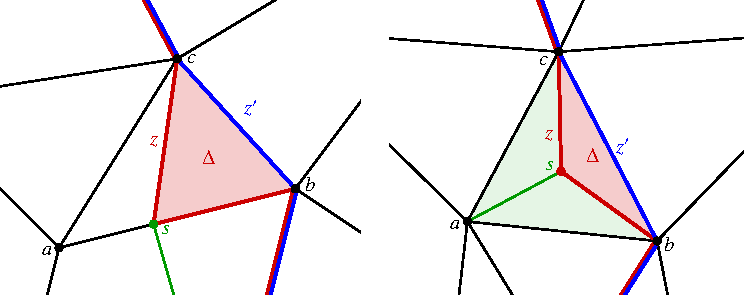
\includegraphics{chapters/120-topologie/images/unterzyklen.pdf}
\caption{Unterteilung eines simplizialen Komplexes mit einem neuen Punkt $s$
auf einer Kante (links) bzw.~im Inneren (rechts) eines 2-Simplex.
Ein Zyklus $z$, der die neue Kante $cs$ verwendet, verwendet auch eine der
neuen Kanten $as$ oder $sb$ ($sb$ im gezeichneten Fall).
Subtraktion des Randes von $\Delta$ verwandelt $z$ in $z-\partial\Delta = z'$.
$z$ und $z'$ sind daher homolog, der Zyklus $z$ ist keine neue
Homologieklasse.
\label{buch:topologie:simplex:fig:unterzyklen}}
\end{figure}
%
Wir müssen zeigen, dass das Hinzufügen eines Unterteilungspunktes 
die einzelnen Vektorräume nicht ändert.
Wir werden keinen vollständigen formellen Beweis geben, sondern
nur anhand einiger Fälle illustrieren, dass die durch den eingefügten
Punkt entstandenen neuen Zyklen homolog sind zu bereits vorhandenen.

Die Unterteilung einer Kante $a_0a_1$ mit einem neuen Punkt $b$ erzeugt
zwei neue Kanten $a_0b$ und $ba_1$.
Da $b-a_0=\partial (a_0b)$ ein Rand ist, sind die Vektoren $a_0\in H_0$
und $b\in H_0$ homolog.
Insbesondere hat sich $H_0$ durch den neuen Punkt nicht verändert.

Ein Unterteilungspunkt $s$ auf einer Kante eines Dreiecks $abc$ fügt auch
eine neu Kante ein, die den neuen Punkt mit dem gegenüberliegenden
Punkt des Dreiecks verbindet.
Die beiden Hälften des Dreiecks haben als Rand jeweils einen Zyklus,
der die neue Kante enthält.

Nehmen wir an, dass diese neue Kante Teil eines Zyklus $z$ ist
(in Abbildung~\ref{buch:topologie:simplex:fig:unterzyklen} links
die Kante $cs$).
Dann muss der Zyklus auch eine der halben Kanten enthalten (den
Teil $sb$ in der Abbildung).
Indem wir den Rand des Dreiecks $\Delta$ subtrahieren, welches die gleiche
halbe Kante enthält, verschwindet sowohl die neue Kante wie auch die
halbe Kante aus dem Zyklus $z$, $z'=z-\partial\Delta$.
Indem wir diese Operation wenn nötig mehrmals durchführen, erhalten
wir einen homologen Zyklus, der im nicht unterteilten Zellenkomplex
liegt.
Das Hinzufügen eines Unterteilungspunktes hat also nur neue Zyklen
hinzugefügt, die homolog sind zu bereits bekannten.

Wir unterteilen jetzt das Dreieck $abc$ mit dem inneren Punkt $s$
(Abbildung~\ref{buch:topologie:simplex:fig:unterzyklen} rechts).
Es entstehen drei neue Dreiecke $abs$, $bcs$ und $cas$ und drei neue
Kanten $as$, $bs$ und $cs$ (in der Abbildung {\color{darkgreen}grün}
eingezeichnet).
Wenn ein Zyklus ${\color{darkred}z}$ im unterteilten $Z_1$ eine der
neuen Kanten enthält, dann muss er auch noch eine weitere solche
Kanten enthalten (die Kanten $cs$ und $bs$ in der Abbildung).
Die beiden Kanten gehören zu genau einem der neuen Dreiecke ($\Delta$
in der Abbildung).
Indem man den Rand dieses Dreiecks vom Zyklus $z$ subtrahiert, erhält
man einen homologen Zyklus $z'=z-\partial\Delta$, der die neuen Kanten
nicht mehr braucht.

Als letztes Beispiel unterteilen wir ein Tetraeder $abcd$ mit
einem inneren Punkt $p$ (Abbildung~\ref{buch:topologie:simplex:fig:zyklus}).
%
% fig-zyklus.tex
%
% (c) 2025 Prof Dr Andreas Müller
%
\begin{figure}
\centering
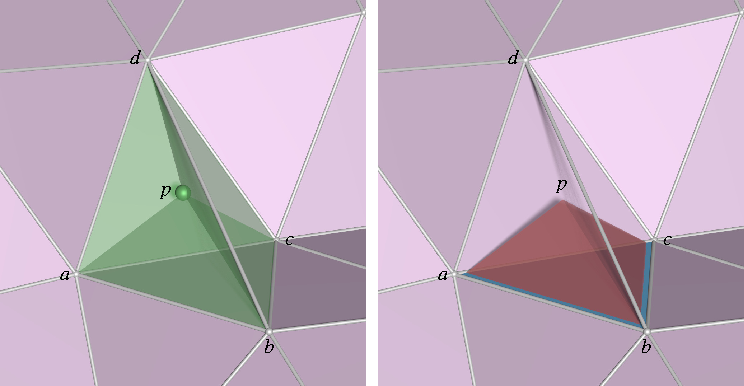
\includegraphics{chapters/120-topologie/images/zyklus.pdf}
\caption{Unterteilung des 3-Simplex $abcd$ mit dem inneren Punkt $p$
(links).
Es entstehen sechs neue 2-Simplizes ({\color{darkgreen}grün}) und vier
neue 3-Simplizes, die durch jeweils drei neue und ein ursprüngliches
2-Simplex berandet sind.
Wenn ein Zyklus (die hellrot dargestellten 2-Simplizes der ``Rückwand'')
eines der neuen 2-Simplizes enthält, dann enthält
er auch noch zwei andere, die eines der vier 3-Simplizes beranden
(rechts, rotes 3-Simplex).
Durch subtrahieren des Randes dieses 3-Simplex bleibt nur
wird der Zyklus auf einen homologen Zyklus mit dem blauen 2-Simplex
reduziert.
\label{buch:topologie:simplex:fig:zyklus}}
\end{figure}
%
Dabei entstehen zu jeder Seitenfläche des Tetraeders ein neues 
Tetraeder und insgesamt sechs neue 2-Simplizes (in der Abbildung
grün dargestellt).
Je zwei der Tetraeder haben jeweils ein neues Dreieck als Seitenfläche
gemeinsam, und je drei eine neue Kante.
Wenn ein Zyklus $z\in Z_2$ eines der neuen Dreieck enthält, dann
muss er auch zwei weitere der neuen Dreiecke enthalten.
Diese drei Dreiecke bestimmen genau eines der neuen Tetraeder.
Subtrahiert man diese Tetraeder von $z$, erhält man einen neuen
Zyklus, der $p$ nicht mehr enthält.
Jeder Zyklus im verfeinerten Zellenkomplex ist also homolog
zu einem Zyklus im ursprünglichen Komplex.
\end{proof}

Der Satz bedeutet, dass die Homologievektorräume mit Hilfe einer
beliebigen Triangulation berechnet werden können.

\begin{beispiel}
\label{buch:topologie:euler:beispiel:tetraeder}
Ein (hohles) Tetraeder $T$ hat vier Ecken, sechs Kanten und vier Seitenflächen.
Das es zusammenhängend ist, wissen wir bereits, dass
$H_0(T,\mathbb{R})=\mathbb{R}$ ist.

Ein eindimensionaler Zyklus ist ein geschlossener Weg.
Enthält ein solcher Weg zwei aneinanderstossende Kanten, dann kann
man den Rand des zugehörige Dreiecks subtrahieren und erhält
einen homologen Zyklus mit einer Kante weniger.
Wiederholung des Prozesses zeigt, dass jeder Zyklus zu 0 homolog
ist, es folgt $H_1(T,\mathbb{R})=0$.

Da das Tetraeder keine dreidimensionalen Simplizes enthält, ist 
$B_2(T)=0$ und folglich $H_2(T,\mathbb{R})=Z_2(T)$.
\end{beispiel}

\begin{beispiel}
\label{buch:topologie:euler:beispiel:kugel}
Da eine Kugel durch Zentralprojektion von einem Tetrader mit
Mittelpunkt im Kugelmittelpunkt trianguliert werden kann, gilt
\[
H_0(S^2,\mathbb{R}) = \mathbb{R},\qquad
H_1(S^2,\mathbb{R}) = 0,\qquad
H_2(S^2,\mathbb{R}) = \mathbb{R}.
\qedhere
\]
\end{beispiel}

%
% fig-torushomologie.tex
%
% (c) 2025 Prof Dr Andreas Müller
%
\begin{figure}
\centering
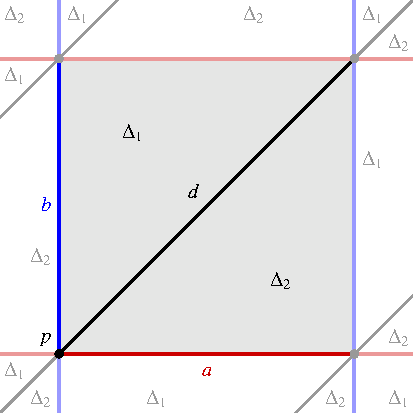
\includegraphics{chapters/120-topologie/images/torushomologie.pdf}
\caption{Triangulation eines Torus mit genau einer Ecke $p$, drei
Kanten $a$, $b$ und $d$ und zwei Dreiecken $\Delta_1$ und $\Delta_2$.
\index{Torus}%
\index{Triangulation}%
Die Kanten gleicher Farbe sind jeweils miteinander zu identifizieren,
sie entsprechen den Kurven gleicher Farbe in
\index{Kurve}%
Abbildung~\ref{buch:topologie:intro:fig:torus}.
\label{buch:topologie:euler:fig:torushomologie}}
\end{figure}
%

\begin{beispiel}
\label{buch:topologie:euler:beispiel:torus}
Zur Berechnung der Homologievektorräume eines zweidimensionalen
Torus $T^2$ lassen sich mit der Triangulation von
Abbildung~\ref{buch:topologie:euler:fig:torushomologie} bestimmen.
Sie enthält genau eine Ecke $p$, drei Kanten $a$, $b$ und $d$ und
zwei Dreiecke $\Delta_1$ und $\Delta_2$.
Die gleichfarbigen Kanten sind jeweils miteinander zu identifizieren.
Sie entsprechen den farbigen Kurven auf dem Torus von
Abbildung~\ref{buch:topologie:intro:fig:torus}.

Da der Torus zusammenhängend ist, ist $H_0(T^2,\mathbb{R})=\mathbb{R}$.

Zwei eindimensionale Zyklen sind leicht zu identifizieren: die 
horizontalen und vertikalen Kanten.
Die diagonale Kante ist homolog zur Verkettung der anderen beiden,
so dass $H_1(T^2,\mathbb{R})$ ein zweidimensionaler Vektorraum
mit den beiden farbigen Kanten als Basis ist.
Somit ist $H_2(T^2,\mathbb{R})=\mathbb{R}^2$.

Da $T^2$ keine dreidimensionalen Simplizes enthält, ist $B_2(T^2)=0$
und folglich $H_2(T^2,\mathbb{R}) = Z_2(T^2)$.
Ein zweidimensionaler Zyklus, der das eine Dreieck enthält, muss auch
das andere enthalten, damit sich die Ränder in der Summe wegheben.
Somit ist $\Delta_1 + \Delta_2$ der einzige Zyklus und es folgt
$H_2(T^2,\mathbb{R})=\mathbb{R}$.
\end{beispiel}

%
% Betti-Zahlen und Euler-Charakteristik
%
\subsection{Betti-Zahlen und Euler-Charakteristik
\label{buch:topologie:simplex:subsection:betti-euler}}
Die Homologievektorräume codieren Information über einen Zellenkomplex,
die wie die Euler-Charakteristik nicht von einer Verfeinerung
abhängt.
Es ist daher nicht unverschämt zu erwarten, dass sich die Euler-Charakteristik
aus den Homologievektorräumen bestimmen lässt.
Dies soll in diesem Abschnitt gezeigt werden.

%
% Betti-Zahlen
%
\subsubsection{Betti-Zahlen}
Die Homologievektorräume sind endlichdimensionale Vektorräume.
Ihre Dimension sagt etwas über die Komplexität des Zellenkomplexes
aus und verdient daher einen eigenen Namen.

\begin{definition}[Betti-Zahlen]
\index{Betti-Zahl}
Die $k$-te \emph{Betti-Zahl} $\beta_k$ ist die Dimension
\[
\beta_k
=
\dim H_k(S,\mathbb{R}).
\]
\end{definition}

\begin{satz}
Eine Unterteilung des Zellenkomplexes ändert die Betti-Zahlen nicht.
\end{satz}

\begin{proof}
Gemäss Satz~\ref{buch:topologie:eulercharakteristik:satz:homologieunterteilung}
ändert die Unterteilung die Homologie-Vektorräume nicht, also ändert sich
auch deren Dimension nicht.
\end{proof}

\begin{beispiel}
\label{buch:topologie:euler:beispiel:betti-tetraeder}
Im Beispiel~\ref{buch:topologie:euler:beispiel:tetraeder} wurden die 
Homologievektorräume eines Tetraeders und anschliessend in
Beispiel~\ref{buch:topologie:euler:beispiel:kugel} einer Kugel berechnet.
Daraus lassen sich die Bettizahlen
\[
\beta_0(T) = \beta_0(S^2) = 1,\qquad
\beta_1(T) = \beta_1(S^2) = 0,\qquad
\beta_2(T) = \beta_2(S^2) = 1
\]
ablesen.
\end{beispiel}

\begin{beispiel}
\label{buch:topologie:euler:beispiel:betti-torus}
Im Beispiel~\ref{buch:topologie:euler:beispiel:torus} wurden die 
Homologievektorräume eines Torus $T^2$ berechnet.
Daraus lassen sich die Bettizahlen
\[
\beta_0(T^2) = 1,\qquad
\beta_1(T^2) = 2,\qquad
\beta_2(T^2) = 1
\]
ablesen.
\end{beispiel}

%
% Euler-Charakteristik
%
\subsubsection{Euler-Charakteristik}
Die alternierende Summe der Betti-Zahlen aus den
Beispielen~\ref{buch:topologie:euler:beispiel:betti-tetraeder}
und \ref{buch:topologie:euler:beispiel:betti-torus} ergibt
\begin{align*}
1-0+1 &= 2 \\
1-2+1 &= 0.
\end{align*}
Dies stimmt mit den in
Tabelle~\ref{buch:topologie:intro:table:eulercharakteristik}
protokollierten Euler-Charakteristiken überein.
Dies suggeriert, dass sich die Euler-Charakteristik bereits aus
den Betti-Zahlen bestimmen lässt.
Der folgende Satz zeigt, dass dies tatsächlich möglich ist.

\begin{satz}
\label{buch:topologie:simplex:satz:euler-betti}
Die Euler-Charakteristik ist durch die Betti-Zahlen bestimmt,
es gilt
\[
\chi(S)
=
\sum_{k=0}^n (-1)^k \beta_k.
\]
\end{satz}

\begin{proof}
Die Eulercharakteristik ist als alternierende Summe der Anzahl der Simplizes 
jeder Dimension definiert.
Die Anzahl tritt als Dimension der Vektorräume $C_k$ auf.
$\dim C_0$ ist die Anzahl der Ecken, $\dim C_1$ die Anzahl der Kanten,
$\dim C_2$ die Anzahl der Dreieck usw.
Die Euler-Charakteristik kann man daher auch schreiben als
\[
\chi(S)
=
\sum_{k=0}^n (-1)^k \dim C_k.
\]
Um die Notation zu vereinfachen, schreiben wir für die alternierende
Summe der Betti-Zahlen als
\[
\chi_H(S)
=
\sum_{k=0}^n
(-1)^k \beta_k
=
\sum_{k=0}^n
(-1)^k \dim H_k(S,\mathbb{R}),
\]
wobei die Notation andeuten soll, dass dies die ``homologisch''
definierte Euler-Cha\-rak\-te\-ris\-tik ist.

Die Homologievektorräume sind ebenfalls endlichdimensionale Vektorräume.
Ihre Dimension ergibt sich aus
\[
\dim H_k(S)
=
\dim Z_k(S) - \dim B_k(S).
\]
Die Dimensionen von $Z_k$ und $B_k$ sind aber mit den Dimensionen von
$C_k$ über den Randoperator verbunden.

Die Ränder $B_k$ sind der Bildraum des Operators $\partial_{k+1}$, seine
Dimension wird durch den Rang gegeben:
\begin{equation}
\dim B_k
= 
\operatorname{Rang} \partial_{k+1}.
\label{buch:topologie:simplex:eqn:dimb}
\end{equation}

Die Zyklen $Z_k$ bilden den Kern des Operators $\partial_k$, so dass
die Dimension von $Z_k$
\begin{equation}
\dim Z_k
=
\dim\ker \partial_k
=
\dim C_k - \operatorname{rank} \partial_k
\label{buch:topologie:simplex:eqn:dimz}
\end{equation}
ist.

Aus den Gleichungen folgt jetzt für die Betti-Zahlen
\begin{equation}
\dim H_k(S,\mathbb{R})
=
\dim Z_k - \dim B_k
=
\dim C_k - \operatorname{rank} \partial_k
- \operatorname{rank}\partial_{k+1}.
\label{buch:topologie:simplex:eqn:dimh}
\end{equation}
Daraus kann man jetzt die alternierende Summe der Betti-Zahlen
ausrechnen
\begin{align*}
\chi_H(S)
&=
\sum_{k=0}^n (-1)^k \dim H_k(S,\mathbb{R})
\\
&=
\sum_{k=0}^n (-1)^k\bigl(
\dim C_k - \operatorname{rank} \partial_k
- \operatorname{rank}\partial_{k+1}
\bigr)
\\
&=
\sum_{k=0}^n (-1)^k\dim C_k
-\sum_{k=0}^n(-1)^k\operatorname{rank}\partial_k
-\sum_{k=1}^n(-1)^k\operatorname{rank}\partial_{k+1}.
\intertext{Die erste Summe ist die Euler-Charakteristik.
In der letzten Summe verschieben wir den Summationsindex um 1 und
erhalten die leichter zu vergleichenden Summen}
&=
\chi(S)
-\sum_{k=0}^n(-1)^k\operatorname{rank}\partial_k
+\sum_{k=1}^{n+1}(-1)^{k}\operatorname{rank}\partial_{k}.
\intertext{Bis auf den ersten Term der linken Summe und den letzten Term
der rechten Summe haben sich die Terme der beiden Summen gegenseit weg,
so dass nur}
&=
\chi(S)
-\operatorname{rank}\partial_0
+(-1)^{n+1}\operatorname{rank}\partial_{k+1}
\end{align*}
übrig bleibt.
Der Operator $\partial_0$ ist aber der Nulloperator und hat daher Rang 0.
Da $S$ ein $n$-dimensionaler Zellenkomplex ist, gibt es keine
$(n+1)$-Zyklen.
Somit ist auch $\partial_{n+1}=0$ und $\operatorname{rank}\partial_{n+1}=0$
und damit $\chi_H(S) = \chi(S)$.
\end{proof}

Es ist daher durchaus gerechtfertigt, einem Kettenkomplex $C=(C_*,\partial_*)$
eine Euler-Charakteristik 
\[
\chi(C)
=
\chi(C_*,\partial_*)
=
\sum_{k\in\mathbb{N}} (-1)^k\dim H_k(C)
\]
zuzuordnen.
\index{Euler-Charakteristik!eines Kettenkomplexes}%
Der Satz~\ref{buch:topologie:simplex:satz:euler-betti}
zeigt dann, dass die früher definierte Euler-Charakteristik des
Zellenkomplexes dasselbe ist wie die Euler-Charakteristik des
zugehörigen Kettenkomplexes.
Der eben gelieferte Beweis des
Satz~\ref{buch:topologie:simplex:satz:euler-betti}
zeigt ausserdem, dass diese Euler-Charakteristik eines beliebigen
Kettenkomplexes, unabhängig davon, ob er als Kettenkomplex eines
Zellenkomplexes gefunden wurde, ebenfalls als alternierende Summe
\[
\chi(C)
=
\sum_{k\in\mathbb{N}} (-1)^k \dim C_k
\]
berechnet werden kann, wenigstens wenn die Vektorräume $C_k$ alle
endlichdimensional sind.




